% Non-technical overview (same style as architecture.tex), for the CIO -> CEO presentation.
% Build: latexmk -pdf ceo-overview.tex
\documentclass[tikz,border=4pt]{standalone}
\usepackage[T1]{fontenc}
\usepackage{helvet}
\renewcommand{\familydefault}{\sfdefault}
\usetikzlibrary{positioning,fit,arrows.meta,calc,backgrounds}

\definecolor{awsB}{HTML}{C76A00}\definecolor{awsF}{HTML}{FFF6EA}
\definecolor{gcpB}{HTML}{1A5FC8}\definecolor{gcpF}{HTML}{EEF4FE}
\definecolor{stoF}{HTML}{E9F6EC}\definecolor{stoB}{HTML}{2E7D32}
\definecolor{cmpF}{HTML}{F3EEFB}\definecolor{cmpB}{HTML}{6A4BA8}
\definecolor{extF}{HTML}{F2F2F2}\definecolor{extB}{HTML}{555555}
\definecolor{flow}{HTML}{C62828}\definecolor{rep}{HTML}{00796B}
\definecolor{ben}{HTML}{2E7D32}

\tikzset{
  font=\small,
  box/.style={draw=#1, rounded corners=3pt, align=center, inner sep=3pt, line width=0.6pt},
  ctl/.style={box=black!60, fill=white, minimum height=1.25cm},
  sto/.style={box=stoB, fill=stoF, minimum height=1.1cm},
  cmp/.style={box=cmpB, fill=cmpF, minimum height=1.25cm},
  ext/.style={box=extB, fill=extF, minimum height=1.1cm},
  arr/.style={-{Stealth[length=5pt]}, line width=0.8pt},
  biarr/.style={{Stealth[length=5pt]}-{Stealth[length=5pt]}, line width=0.8pt},
  stepn/.style={circle, fill=flow, text=white, inner sep=1pt, font=\scriptsize\bfseries},
  bnf/.style={rectangle, rounded corners=2pt, fill=ben, text=white, inner sep=2pt, font=\scriptsize\bfseries},
  lbl/.style={font=\scriptsize, align=center, inner sep=1pt},
}

\begin{document}
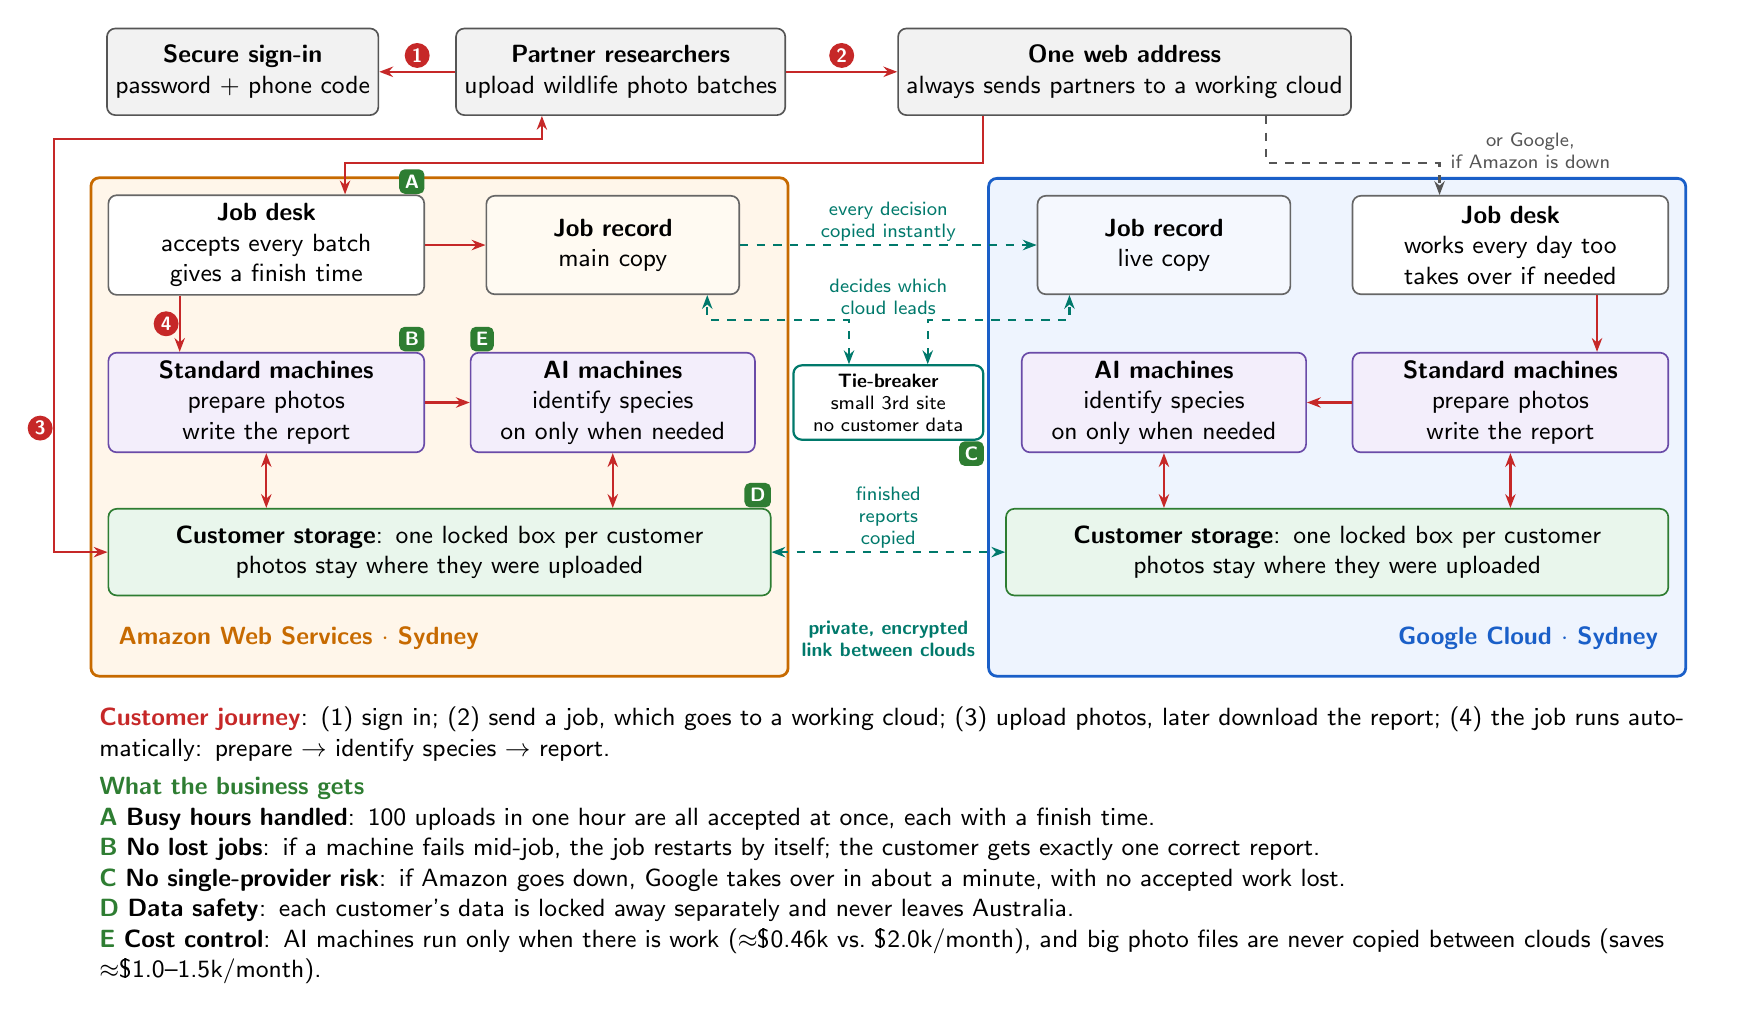
\begin{tikzpicture}

% ================= top row
\node[ext, minimum width=3.4cm] (idp) at (2.0,10.1)
  {\textbf{Secure sign-in}\\password + phone code};
\node[ext, minimum width=3.8cm] (users) at (6.8,10.1)
  {\textbf{Partner researchers}\\upload wildlife photo batches};
\node[ext, minimum width=5.0cm] (dns) at (13.2,10.1)
  {\textbf{One web address}\\always sends partners to a working cloud};

% ================= AWS (left)
\node[ctl, text width=3.8cm] (jobA) at (2.3,7.9)
  {\textbf{Job desk}\\accepts every batch\\gives a finish time};
\node[ctl, text width=3.0cm, fill=awsF!60] (dbA) at (6.7,7.9)
  {\textbf{Job record}\\main copy};
\node[cmp, text width=3.8cm] (cpuA) at (2.3,5.9)
  {\textbf{Standard machines}\\prepare photos\\write the report};
\node[cmp, text width=3.4cm] (gpuA) at (6.7,5.9)
  {\textbf{AI machines}\\identify species\\on only when needed};
\node[sto, text width=8.2cm] (s3) at (4.5,4.0)
  {\textbf{Customer storage}: one locked box per customer\\photos stay where they were uploaded};
\node[anchor=west, align=left] (noteA) at (0.3,2.9)
  {\textbf{\textcolor{awsB}{Amazon Web Services $\cdot$ Sydney}}};
\begin{scope}[on background layer]
\node[box=awsB, fill=awsF, line width=1pt, fit=(jobA)(dbA)(cpuA)(gpuA)(s3)(noteA), inner sep=6pt] (aws) {};
\end{scope}

% ================= Google Cloud (right, mirrored: x' = 20.4 - x)
\node[ctl, text width=3.8cm] (jobG) at (18.1,7.9)
  {\textbf{Job desk}\\works every day too\\takes over if needed};
\node[ctl, text width=3.0cm, fill=gcpF!60] (dbG) at (13.7,7.9)
  {\textbf{Job record}\\live copy};
\node[cmp, text width=3.8cm] (cpuG) at (18.1,5.9)
  {\textbf{Standard machines}\\prepare photos\\write the report};
\node[cmp, text width=3.4cm] (gpuG) at (13.7,5.9)
  {\textbf{AI machines}\\identify species\\on only when needed};
\node[sto, text width=8.2cm] (gcs) at (15.9,4.0)
  {\textbf{Customer storage}: one locked box per customer\\photos stay where they were uploaded};
\node[anchor=east, align=right] (noteG) at (20.1,2.9)
  {\textbf{\textcolor{gcpB}{Google Cloud $\cdot$ Sydney}}};
\begin{scope}[on background layer]
\node[box=gcpB, fill=gcpF, line width=1pt, fit=(jobG)(dbG)(cpuG)(gpuG)(gcs)(noteG), inner sep=6pt] (gcp) {};
\end{scope}

% ================= tie-breaker (third site)
\node[box=rep, fill=white, line width=0.8pt, text width=2.2cm, font=\scriptsize] (wit) at (10.2,5.9)
  {\textbf{Tie-breaker}\\small 3rd site\\no customer data};
\draw[dashed, rep, biarr] (wit.north -| 9.7,0) |- (7.9,6.95) -- (dbA.south -| 7.9,0);
\draw[dashed, rep, biarr] (wit.north -| 10.7,0) |- (12.5,6.95) -- (dbG.south -| 12.5,0);
\node[lbl, text=rep, anchor=south] at (10.2,6.98) {decides which\\cloud leads};

% ================= cross-cloud links (teal)
\draw[arr, rep, dashed] (dbA.east) -- node[lbl, above, text=rep] {every decision\\copied instantly} (dbG.west);
\draw[biarr, rep, dashed] (s3.east) -- node[lbl, above, text=rep] {finished\\reports\\copied} (gcs.west);
\node[lbl, text=rep, font=\scriptsize\bfseries] at (10.2,2.9) {private, encrypted\\link between clouds};

% ================= journey (red, numbered)
\draw[arr, flow] (users.west) -- node[stepn, above=1pt] {1} (idp.east);
\draw[arr, flow] (users.east) -- node[stepn, above=1pt] {2} (dns.west);
\draw[arr, flow] (dns.south -| 11.4,0) -- ++(0,-0.6) -| (jobA.north -| 3.3,0);
\draw[arr, extB, dashed] (dns.south -| 15.0,0) -- ++(0,-0.6) -| (jobG.north -| 17.2,0);
\node[lbl, text=extB, anchor=west] at (17.3,9.1) {or Google,\\if Amazon is down};
\draw[biarr, flow] (users.south -| 5.8,0) -- (5.8,9.25) -- (-0.4,9.25) |- node[stepn, pos=0.35, left] {3} (s3.west);
\draw[arr, flow] (jobA.east) -- (dbA.west);
\draw[arr, flow] (jobA.south -| 1.2,0) -- node[stepn, left] {4} (cpuA.north -| 1.2,0);
\draw[arr, flow] (cpuA.east) -- (gpuA.west);
\draw[biarr, flow] (cpuA.south) -- (cpuA.south |- s3.north);
\draw[biarr, flow] (gpuA.south) -- (gpuA.south |- s3.north);
\draw[arr, flow] (jobG.south -| 19.2,0) -- (cpuG.north -| 19.2,0);
\draw[arr, flow] (cpuG.west) -- (gpuG.east);
\draw[biarr, flow] (cpuG.south) -- (cpuG.south |- gcs.north);
\draw[biarr, flow] (gpuG.south) -- (gpuG.south |- gcs.north);

% ================= benefit tags (green)
\node[bnf, anchor=south east] at (jobA.north east) {A};
\node[bnf, anchor=south east] at (cpuA.north east) {B};
\node[bnf, anchor=north east] at (wit.south east) {C};
\node[bnf, anchor=south east] at (s3.north east) {D};
\node[bnf, anchor=south west] at (gpuA.north west) {E};

% ================= legend
\node[anchor=north west, align=left, text width=20.4cm, font=\small] at ($(aws.south west)+(0,-0.25)$)
  {\textcolor{flow}{\textbf{Customer journey}}: (1) sign in; (2) send a job, which goes to a working cloud;
   (3) upload photos, later download the report; (4) the job runs automatically: prepare $\rightarrow$ identify species $\rightarrow$ report.\\[3pt]
   \textcolor{ben}{\textbf{What the business gets}}\\
   \textcolor{ben}{\textbf{A}} \textbf{Busy hours handled}: 100 uploads in one hour are all accepted at once, each with a finish time.\\
   \textcolor{ben}{\textbf{B}} \textbf{No lost jobs}: if a machine fails mid-job, the job restarts by itself; the customer gets exactly one correct report.\\
   \textcolor{ben}{\textbf{C}} \textbf{No single-provider risk}: if Amazon goes down, Google takes over in about a minute, with no accepted work lost.\\
   \textcolor{ben}{\textbf{D}} \textbf{Data safety}: each customer's data is locked away separately and never leaves Australia.\\
   \textcolor{ben}{\textbf{E}} \textbf{Cost control}: AI machines run only when there is work ($\approx$\$0.46k vs.\ \$2.0k/month), and big photo files
   are never copied between clouds (saves $\approx$\$1.0--1.5k/month).};

\end{tikzpicture}
\end{document}
